\documentclass{article}
\usepackage{tikz}
\usetikzlibrary{calc,arrows.meta,shapes.misc,decorations.pathmorphing,backgrounds,positioning,fit}

%graphic for ORI-Book

\begin{document}

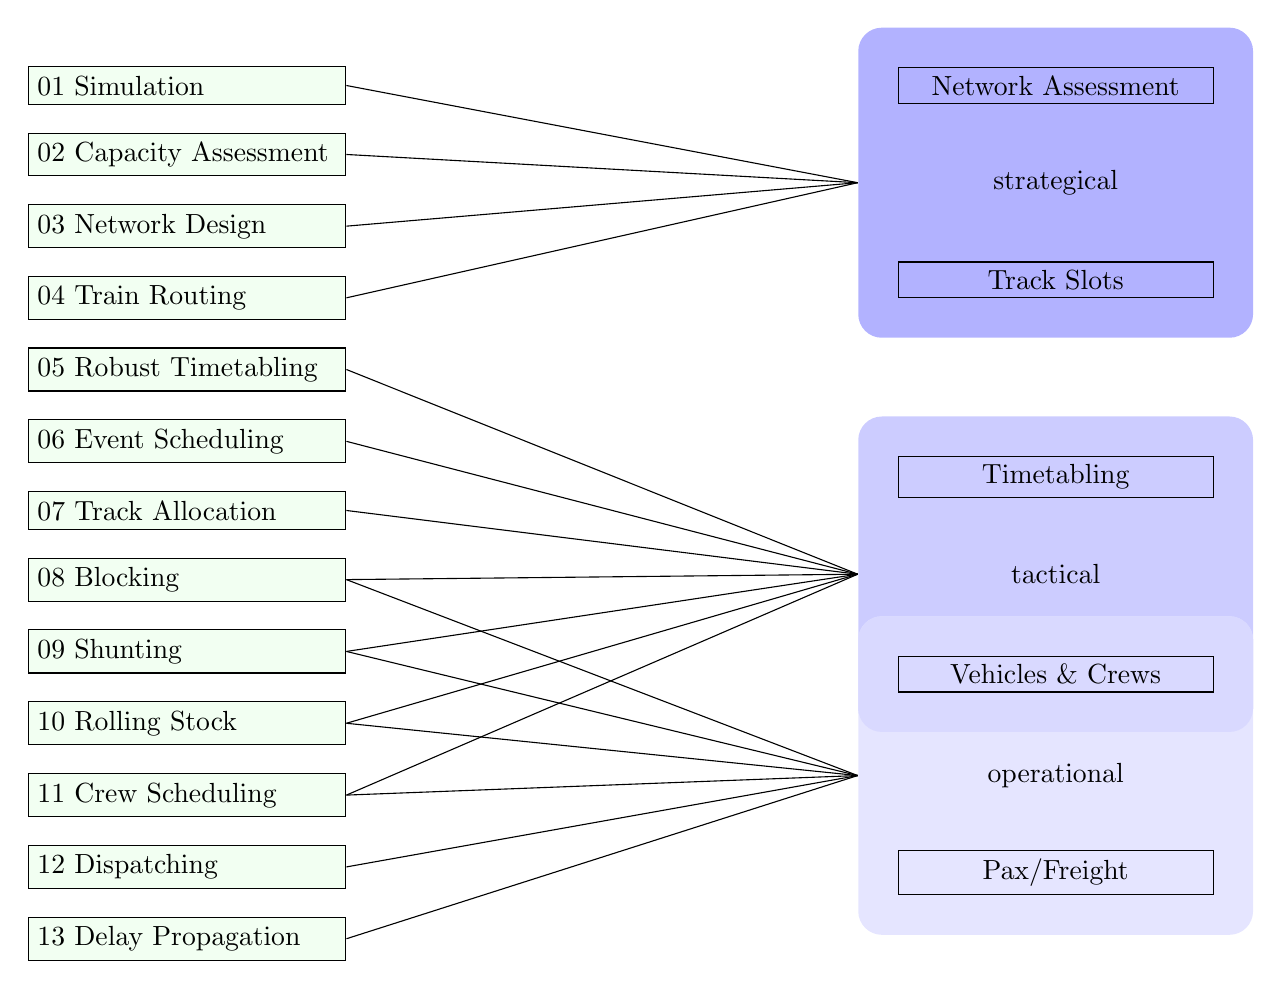
\begin{tikzpicture}
[
chptr/.style={rectangle, fill=green!5, below=1em, minimum width = 4cm, text width=3.8cm, align=left}, 
level/.style={rectangle, rounded corners=3mm, inner sep = .5cm},
topic/.style={rectangle, minimum width = 4cm, below = 2cm, inner sep = 3pt},
>/.tip={Latex[length=7mm, width=.5mm]}]





	\node (sim) at (-5,10) [chptr,draw]{01 Simulation};
	\node (capass) [below=of sim,chptr,draw, align=left]{02 Capacity Assessment};
	\node (ntwd) [below=of capass,chptr,draw]{03 Network Design};
	\node (trou) [below=of ntwd,chptr,draw]{04 Train Routing};
	\node (rott) [below=of trou,chptr,draw]{05 Robust Timetabling};
	\node (evscd) [below=of rott,chptr,draw]{06 Event Scheduling};
	\node (tall) [below=of evscd,chptr,draw]{07 Track Allocation};
	\node (block) [below=of tall,chptr,draw]{08 Blocking};
	\node (shu) [below=of block,chptr,draw]{09  Shunting};
	\node (rosto) [below=of shu,chptr,draw]{10 Rolling Stock};
	\node (cscd) [below=of rosto,chptr,draw]{11 Crew Scheduling};
	\node (disp) [below=of cscd,chptr,draw]{12  Dispatching};
	\node (delpp) [below=of disp,chptr,draw]{13  Delay Propagation};
	
	
	\node (nw)  [topic,right=7cm of sim,draw] {Network Assessment};		
	\node  (ts) [below=of nw,topic,draw] {Track Slots};
	\node (tt) [below=of ts,topic,draw] {Timetabling};
	\node (vc) [below=of tt,topic,draw]{Vehicles \& Crews};
	\node (pf) [below=of vc,topic,draw]{Pax/Freight};
	%\node (test) [draw, below=of ts, shape=rounded rectangle]{test};	 
		 
	\begin{scope}[on background layer]
	
	\node (strat) [level,fill=blue!30,fit=(nw) (ts)]{};
	%\node (labstrat) [rotate=-90,right=.5cm of strat,blue!30,draw]{strategical};
	
	\node (tact) [level,fill=blue!20,fit= (tt) (vc), save path=\nodepatha]{};
	%\node (labtact) [right=0.5cm of tact,blue!30]{tactical};
	
	\node (op) [level, fill=blue!10,fit= (vc) (pf), save path=\nodepathb]{};
	%\node (labop) [right=0.5cm of op,blue!30, rotate=-90]{operational};
	
	
	\begin{scope}
             \path [clip] \pgfextra{\pgfsetpath\nodepatha};
            \fill [blue!15] \pgfextra{\pgfsetpath\nodepathb}; 
 	 \end{scope}
	 
	\node[rotate = 0] (labstrat) at (strat) {strategical};
	\node[rotate = 0] (labtact) at (tact) {tactical};
	\node[rotate = 0] (labop) at (op) {operational};
		
	\end{scope}
	
	\coordinate (tactin) at ($(tact.west) + (0,0)$);
	\coordinate (stratin) at ($(strat.west) + (0,0)$);
	\coordinate (opin) at ($(op.west) + (0,0)$);
	
	\draw[-] (sim.east) -- (stratin);
	\draw[-] (capass.east) -- (stratin);
	\draw[-] (ntwd.east) -- (stratin);
	\draw[-] (trou.east) -- (stratin);
	\draw[-] (rott.east) -- (tactin);
	\draw[-] (evscd.east) -- (tactin);
	\draw[-] (tall.east) -- (tactin);
	\draw[-] (block.east) -- (tactin);
	\draw[-] (block.east) -- (opin);
	\draw[-] (shu.east) -- (tactin);
	\draw[-] (shu.east) -- (opin);
	\draw[-] (rosto.east) -- (tactin);
	\draw[-] (rosto.east) -- (opin);
	\draw[-] (cscd.east) -- (tactin);
	\draw[-] (cscd.east) -- (opin);
	\draw[-] (disp.east) -- (opin);
	\draw[-] (delpp.east) -- (opin);
	
	
	  
\end{tikzpicture}

\end{document}
